\begin{figure}[htb!]
	\centering
	\footnotesize

	\psfrag{a}[c][c] {$5$}
	\psfrag{b}[c][c] {$1$}
	\psfrag{c}[c][c] {$2$}

	\psfrag{d}[c][c] {$0$}
	\psfrag{e}[c][c] {$-1$}
	\psfrag{f}[c][c] {$0$}

	\psfrag{g}[c][c] {$0$}
	\psfrag{h}[c][c] {$1$}
	\psfrag{i}[c][c] {$6$}

	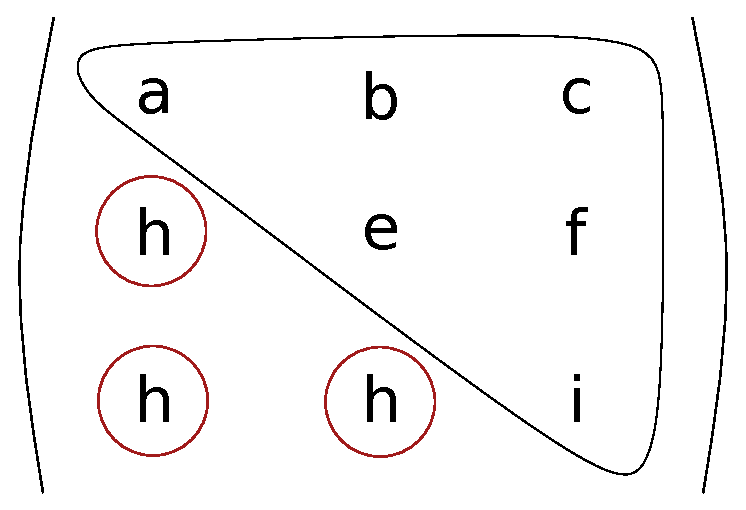
\includegraphics[width=0.4\textwidth]{matrixA213132.eps}
	\caption{The entry $A_{21}$, $A_{31}$, and $A_{32}$ of matrix $A$ are the three entries
		that we would like clean up
		so that we may obtain a right upper triangular matrix.
		Givens-Rotation matrix for $A_{21}$, $A_{31}$, and $A_{32}$ is $G_{21}$, $G_{31}$, and $G_{32}$, respectively.
		The order of applying $G_{21}$ first or $G_{31}$ or $G_{32}$ is no matter, but
		the coefficients used to build the Givens-Rotation matrix $r$, $a$, and $b$
		have to be carefully computed, since they become various
		after every time applying the rotation.}
	\label{\LABEL}
\end{figure}
